%=========================================================

% Here you can choose to compile with or without solutions.
% However, this definition is ignored if you use any
% command from the `Makefile`.
\providecommand{\withSol}{\iftrue}

%=========================================================

\documentclass
[twoside,english,colorbacktitle,accentcolor=tud9c]
{tudexercise}

\usepackage[T1]{fontenc}
\usepackage[latin9]{inputenc}
\usepackage{amstext}
\usepackage{amsmath}
\usepackage{graphicx}
\usepackage{setspace}
\usepackage{multicol}
\usepackage{mathtools}
\usepackage{dsfont}
\usepackage{units}
\usepackage{subfigure}
\usepackage{color}
\usepackage{booktabs}
\usepackage{fancyref}
\usepackage[ngerman,english]{babel}

%=========================================================

\def\homework{1}
\def\homeworkVer{1}
\def\homeworkSolVer{1}
\def\lecture{Robot Learning}
\def\semester{Winter Semester 2017/2018}
\def\prof{Prof. Dr. J. Peters, D. Tanneberg, M. Ewerton}
\def\deadline{Due date: Wednesday, 15 November 2017 (before the lecture)}
\graphicspath{{code/}}
%=========================================================

\ifcsname withSol\endcsname\else
  \expandafter\let\csname withSol\expandafter\endcsname
                  \csname iffalse\endcsname
\fi

\withSol
	\usepackage[solutions]{iasHomework}
\else
	\usepackage{iasHomework}
\fi

%=========================================================

\newcommand{\studentdata}{Johannes Beck, 2948911 \qquad Martin Steinborn, 2253402}
%\newcommand{\studentdata}{John Doe, 1234567 \qquad Jane Doe, 7654321}

\begin{document}
	
	\hwtitle{}
	\maketitle
	
	\begin{examheader}
		\normalsize
		\vspace{-1em}
		Name, Surname, ID Number \hfill \studentdata{}
		\vspace{-1em}
	\end{examheader} 
	
	\textbf{Name, Surname, ID Number \hfill \studentdata{}}
	
	%---------------------------------------------
%---------------------------------------------
%---------------------------------------------
%---------------------------------------------
\exercise{Robotics in a Nutshell}
You are considering to buy a new multi-purpose robot platform. Its kinematic chain has two rotational $q_{\{1,3\}}$ and two linear $q_{\{2,4\}}$ degrees of freedom (DoFs), as shown in the figure below. These four joints are actuated with forces and torques of $u_i$, $i\in\{1,2,3,4\}$. A gripper is mounted on the end of the robot, indicated by the letter \textbf{E}. The robot's base is mounted on a table. We assume that the base Cartesian coordinates at the mount are $x_\textrm{base}=[0,0,0]$.  

\begin{center}
  % \includegraphics[width=0.35\textwidth]{fig/S-bot_B} 
\end{center}


\begin{questions}

%----------------------------------------------

\begin{question}{Forward Kinematics}{2}
Compute the kinematic transformation in the global coordinate system from the base $\vec{x_\textrm{base}}$ to the end-effector \textbf{E}.  
Write the solution for the $\vec{x_\textrm{end-eff}}=[x,y,z]^T$  according to the joint values $q_i$, where $i \in \{1,2,3,4\}$.

\begin{answer}
The kinematic transformation in global coordinates from  $\vec{x_\textrm{base}}$ to the end-effector \textbf{E} can be computed and simplyfied to
\begin{align*}
~^\textrm{base}\!T_{\textrm{end-eff}} &= 
%\begin{bmatrix}
%1 & 0 & 0 & 0 \\
%0 & 1 & 0 & 0 \\
%0 & 0 & 1 & \textrm{l}_{\textrm{1}} \\
%0 & 0 & 0 & 1 
%\end{bmatrix}
%\cdot [...]\\ 
%TODO: restliche Matrizen auch aufschreiben?
\begin{bmatrix}
\cos(\textrm{q}_{\textrm{1}}+\textrm{q}_{\textrm{3}}) & -\sin(\textrm{q}_{\textrm{1}}+\textrm{q}_{\textrm{3}})& 0 & \textrm{q}_{\textrm{4}}\cos(\textrm{q}_{\textrm{1}}+\textrm{q}_{\textrm{3}}) + \textrm{q}_{\textrm{2}}\cos(\textrm{q}_{\textrm{1}}) \\
\sin(\textrm{q}_{\textrm{1}}+\textrm{q}_{\textrm{3}}) &\cos(\textrm{q}_{\textrm{1}}+\textrm{q}_{\textrm{3}})  & 0 & \textrm{q}_{\textrm{4}}\sin(\textrm{q}_{\textrm{1}}+\textrm{q}_{\textrm{3}}) + \textrm{q}_{\textrm{2}}\sin(\textrm{q}_{\textrm{1}}) \\
0 & 0 & 1 & \textrm{l}_{\textrm{1}} \\
0 & 0 & 0 & 1 
\end{bmatrix}
\end{align*}.

With that the position of the end-efector $\vec{x_\textrm{end-eff}}=[x,y,z]^T$ results to

\begin{align*}
\vec{x_\textrm{end-eff}}=[x,y,z]^T = \begin{bmatrix}
\textrm{q}_{\textrm{4}}\cos(\textrm{q}_{\textrm{1}}+\textrm{q}_{\textrm{3}}) + \textrm{q}_{\textrm{2}}\cos(\textrm{q}_{\textrm{1}}) \\
\textrm{q}_{\textrm{4}}\sin(\textrm{q}_{\textrm{1}}+\textrm{q}_{\textrm{3}}) + \textrm{q}_{\textrm{2}}\sin(\textrm{q}_{\textrm{1}}) \\
\textrm{l}_{\textrm{1}} 
\end{bmatrix}
\end{align*}.

\end{answer}
\end{question}

%----------------------------------------------

\begin{question}{Inverse Kinematics}{2}
Define briefly in your own words the inverse kinematics problem in robotics.  
Can we always accurately model the inverse kinematics of a robot with a
function?

\begin{answer}
The problem with the inverse kinematics is that the calculation for the parameters is very costly because you have to solve a non-linear equation system each step. This is why in a lot of cases the only way to solve this is a numerical solution but not a analytical(funciton). Also there are often multiple possible solutions for a robot to reach a specific position. So therefor a solution in form of a function isn't even possible.
\end{answer}

\end{question}

%----------------------------------------------

\begin{question}{Differential Kinematics}{4}
Compute the Jacobian matrix $\vec{J}(\vec{q})$ of the robot such that $\dot{\vec{x}}=\vec{J}(\vec{q})\dot{\vec{q}}$, where $\dot{\vec{q}}$ is the first time derivatives of the state vector $\vec{q}$ of the robot. Explain in a sentence the physical meaning of the Jacobian. 

\begin{answer}
For the differential kinematics we can compute the Jacobian matrix to
\begin{align*}
\vec{J}(\vec{q}) = 
%Jacobian
\begin{bmatrix}
% X --------------------------
-\textrm{q}_{\textrm{4}}\sin(\textrm{q}_{\textrm{1}}+\textrm{q}_{\textrm{3}}) + \textrm{q}_{\textrm{2}}\sin(\textrm{q}_{\textrm{1}}) &
\cos(\textrm{q}_{\textrm{1}}) &
-\textrm{q}_{\textrm{4}}\sin(\textrm{q}_{\textrm{1}}+\textrm{q}_{\textrm{3}})&
\cos(\textrm{q}_{\textrm{1}}+\textrm{q}_{\textrm{3}})\\
% Y --------------------------
\textrm{q}_{\textrm{4}}\cos(\textrm{q}_{\textrm{1}}+\textrm{q}_{\textrm{3}}) + \textrm{q}_{\textrm{2}}\cos(\textrm{q}_{\textrm{1}})&
\sin(\textrm{q}_{\textrm{1}})&
\textrm{q}_{\textrm{4}}\cos(\textrm{q}_{\textrm{1}}+\textrm{q}_{\textrm{3}})&
\cos(\textrm{q}_{\textrm{1}}+\textrm{q}_{\textrm{3}})\\
% Z --------------------------
0 & 0 & 0 & 0 
\end{bmatrix}
\end{align*}
for $\dot{\vec{x}}=\vec{J}(\vec{q})\dot{\vec{q}}$.
%TODO: Describe what the jacobian does

\end{answer}

\end{question}

%----------------------------------------------

\begin{question}{Singularities}{3}
What is the kinematic singularity in robotics? How can you detect it? When does our robotic arm, which was defined above, enter a kinematic singularity?

\begin{answer}
So called kinematic singularities are positions, where the colums of the jabobian matrix become linear dependent. This leads to a loss of degrees of freedom %TODO: Not finished yet

\end{answer}

\end{question}

%----------------------------------------------

\begin{question}{Workspace}{1}
If your task is to sort items placed on a table, would you buy this robot? Briefly justify your answer.

\begin{answer}
We wouldn't buy this robot because its workspace is a plane, parallel to the table(distance L1). So since the robot can't reach any point outside his workspace it isn't able to reach the tableplate. So it can't do it's purpose and therefor is not a good buy for this task.
\end{answer}

\end{question}

\end{questions}

	
	\exercise{Control}
In robotic locomotion it is common to abstract from the robot by using inverted pendulum models.
In this exercise we will use a planar double inverted pendulum to test different control strategies. Our robot can be controlled by specifying the torque $\mathbf{u}=[u_1, u_2]$ of its motors. Consider that in mechanical systems the torque $\vec{u}$ is a function of the joint positions $\vec{q}$, velocities $\dot{\vec{q}}$ and accelerations $\ddot{\vec{q}}$, as given by  
\[
\vec{u}=\vec{M}(\vec{q})\ddot{\vec{q}}+\vec{c}(\vec{q},\dot{\vec{q}})+\vec{g}(\vec{q}), 
\] 
where $\vec{M}$ denotes the inertial matrix, $\vec{c}(\vec{q},\dot{\vec{q}})$ the Coriolis and centripetal forces, and $\vec{g}$ the gravity terms. In the following exercises assume that these terms are given.

For the programming exercises you will use the attached code. 
We provide skeletons for controlling the system either in joint space (\texttt{my\_ctl.py}) or in task space (\texttt{my\_taskSpace\_ctl.py}) and a basic functionality for plotting. You can invoke either mode by running \texttt{jointCtlComp.py} or \texttt{taskCtlComp.py} respectively. 
Attach a printout with plots and a snippet of your source code for each programming exercise. 

\begin{questions}
	
	%----------------------------------------------
	
	\begin{question}{PID Controller}{2}
		What is the form of a proportional-integral-derivative (PID) controller and how could you use it to control a robot, i.e. what physical quantities could you control? Name one positive and one negative aspect of PID controllers.
		
\begin{answer}
A PID controller comes in the form of: \begin{align*}
	u=K_{\textrm{p}} (q_{\textrm{des}} - q) + K_{\textrm{D}} (\dot{q_{\textrm{des}}} - \dot{\textrm{q}}) + K_{\textrm{I}} \int_{-\infty}^{t}(q_{\textrm{des}} - q)\textrm{d}\tau
\end{align*}
%TODO:form sentences
With $K_P$ representing the error at the Moment, $K_I$ an accumulation of the past errors and $K_D$ a predictor for future errors based on the current rate of change. 
PID controllers are useful if the robot model is to complex or not known but on the other hand, the end effector will not move to the perfect spot, but will perform a pendulum movement.
%P -> now error\\
%I -> accumulation of past errors\\
%D -> prediction for future error(based on the current rate of change)\\
% positiv: Nuetzlich falls kein gutes model bekannt ist.\\
% negativ: pendelt um gewuenschte position wegen numerischer loesung\\
\end{answer}
		
	\end{question}
	
	%----------------------------------------------
		
	\begin{question}{Gravity Compensation and Inverse Dynamics Control}{4}
		Suppose that you would like to create a control law to set the joint angles on the double inverted pendulum model by controlling the torque of the motors. Write a feedback control law which additionally gravity compensates and then extend it to full inverse dynamics control. 
		
\begin{answer}
	\begin{align*}
		u_t=K_{\textrm{p}} (q_{\textrm{d}} - q_{\textrm{t}}) + K_{\textrm{D}} (\dot{q_{\textrm{d}}} - \dot{\textrm{q}_{\textrm{t}}}) + g(q)
	\end{align*}
	%TODO
\end{answer}
		
	\end{question}
	
	%----------------------------------------------
	
	\begin{question}{Comparison of Different Control Strategies}{12}
		In the following exercise you will investigate the differences of the following control algorithms, P, PID, PD with gravity compensation, and full inverse dynamics.
		The double pendulum is initiated hanging down, with state $\vec{q_\textrm{start}}={[-\pi,0]}$. We simulate the system with a time-step $dt=0.002$ seconds using symplectic Euler integration and run the simulation for $t_\textrm{end}=3s$. 
		
		Implement the control laws by filling the skeleton file \texttt{my\_ctl.py}. Use the following feedback gains $K_P=60, K_D=10, K_I=0.1$ for the first joint and $K_P=30, K_D=6, K_I=0.1$ for the second one.
		The target state of the double pendulum is set to $\vec{q_\textrm{des}}={[-\pi / 2,0]}$. 
		
		Create (max. 4) plots that compare the different control strategies and analyze the results. It is your choice how to illustrate your results. In your analysis you should include a discussion on the overall performance of each controller. Which controllers manage to go to the desired point, and how does the choice of a controller affects the behavior of the second joint of the pendulum? Additionally discuss which controller you would choose and why. The provided code is able to generate plot but feel free to modify it if you like. Points will be deducted for confusing plots. Do not forget to include your source code in your solutions.
		
\begin{answer}
	\begin{center}
	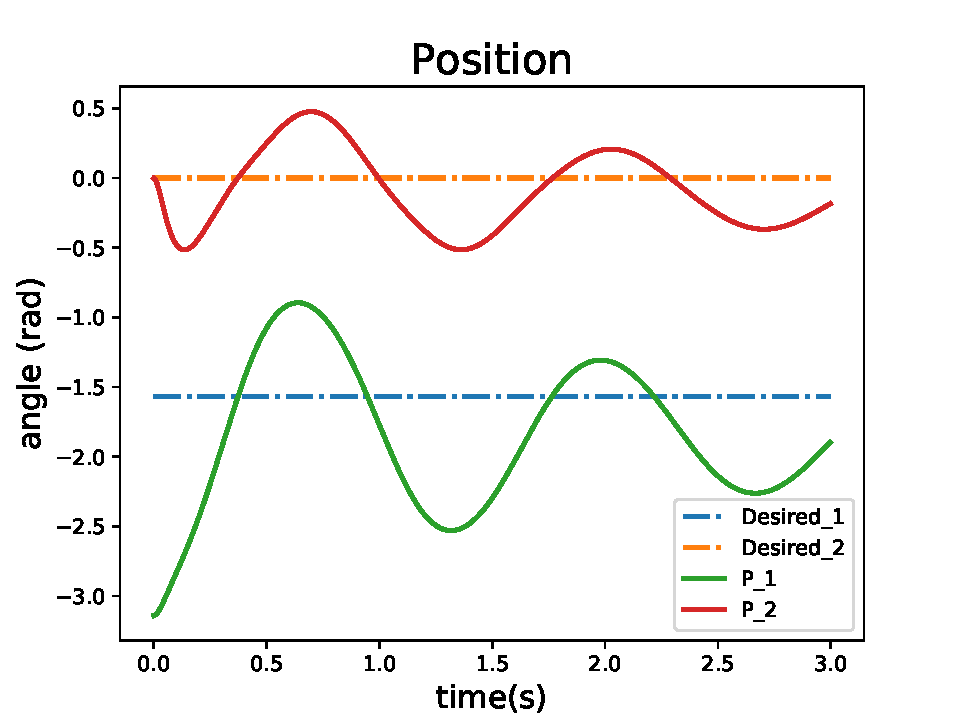
\includegraphics[width=.32\linewidth]{figures/P-Regler0.pdf}
	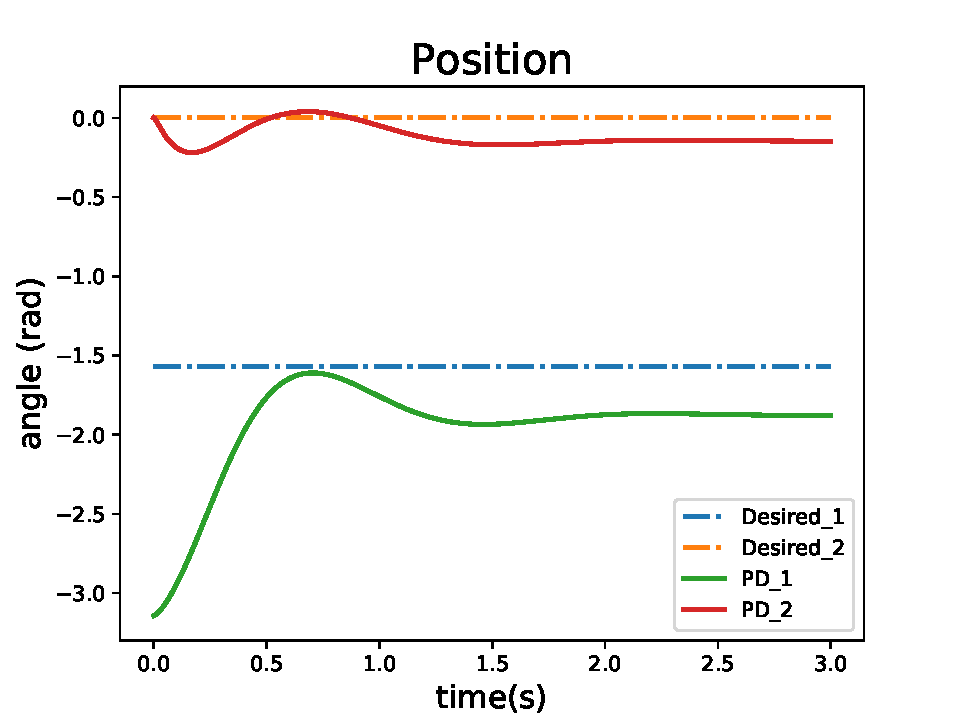
\includegraphics[width=.32\linewidth]{figures/PD-Regler0.pdf}\\
	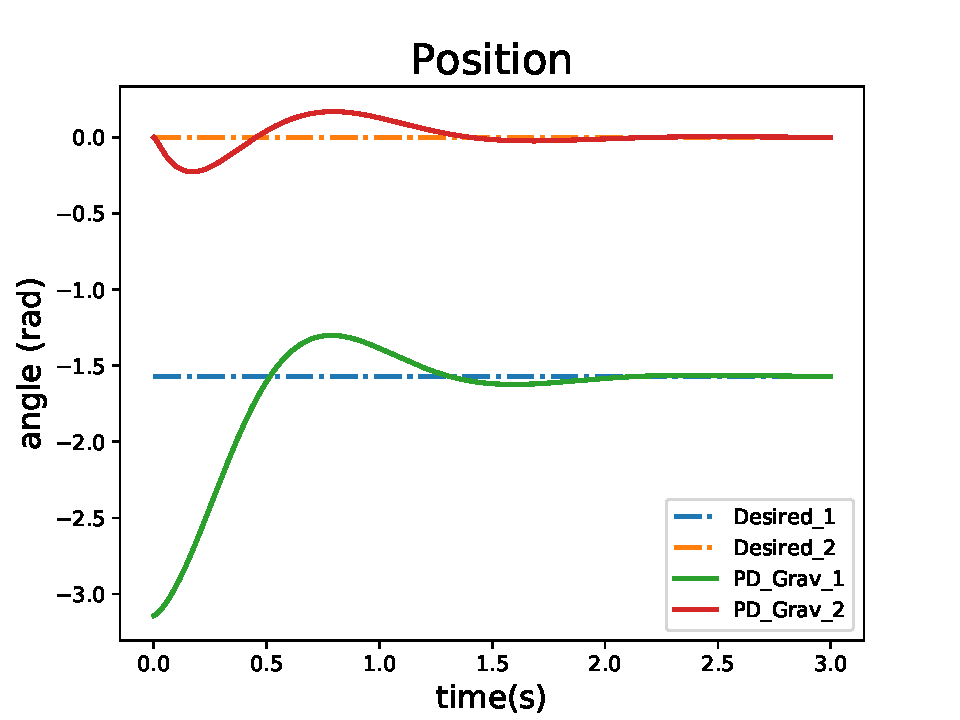
\includegraphics[width=.32\linewidth]{figures/PD-Grav-Regler0.pdf}
	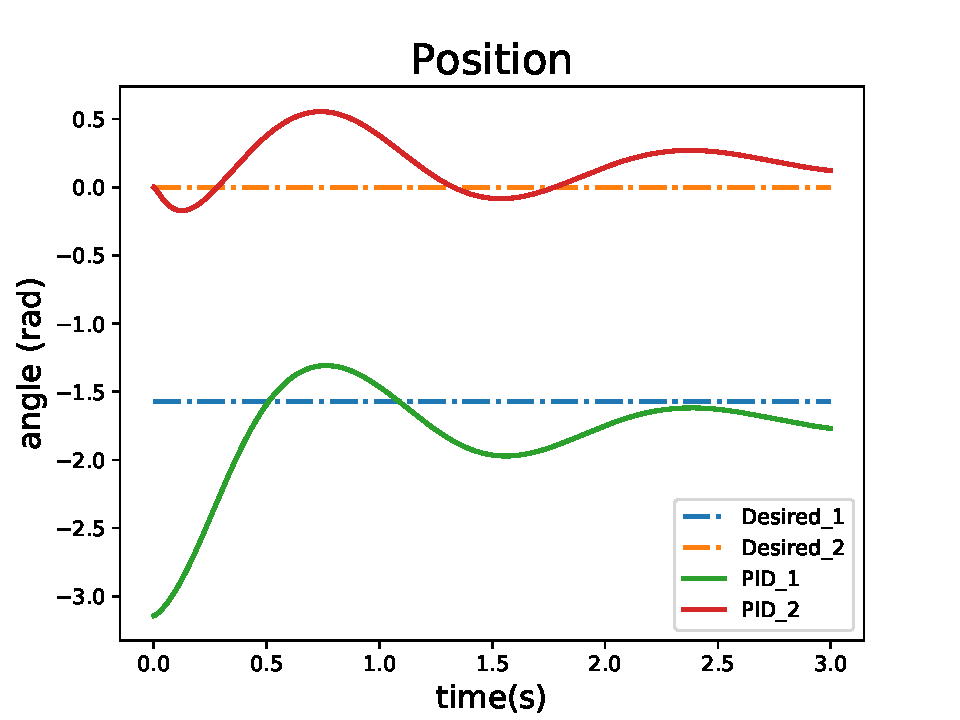
\includegraphics[width=.32\linewidth]{figures/PID-Regler0.pdf}
	%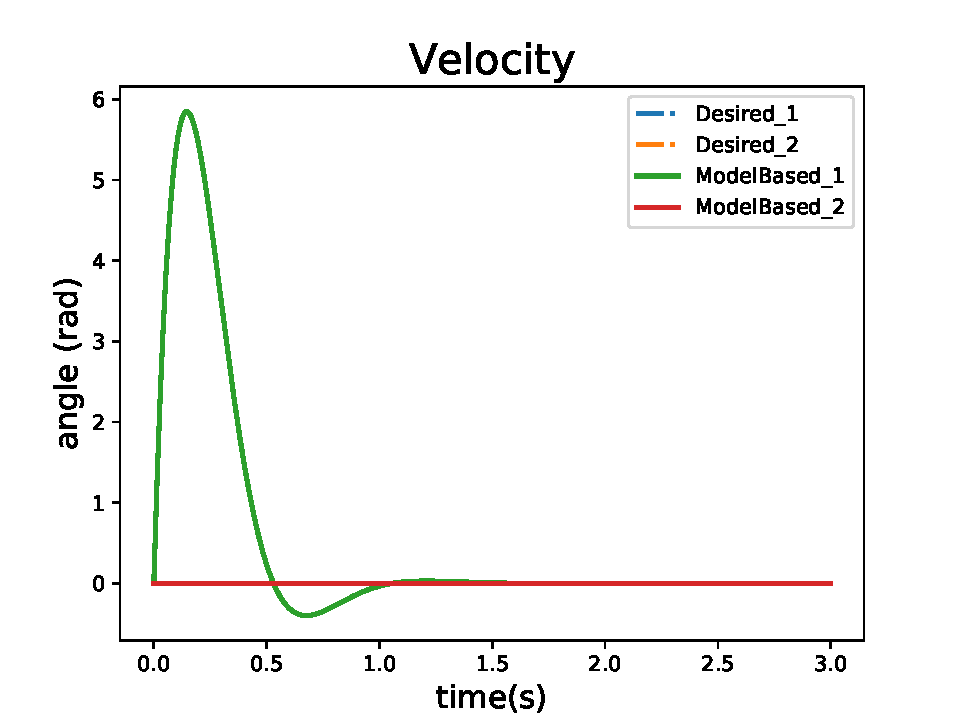
\includegraphics[width=.4\linewidth]{figures/Model-Based-Regler1.pdf}
\end{center}
	The results show that neither the P-controller nor the PID-controller reach the second desired position in the given time frame, on the other hand, it's easy to see that P controller takes a long time to get into the right position, even more it oversteers its destination by way more than the others. The PD controller gets fast to near zero velocity but stays obviously a little bit under his desired position. That's due to gravity, to compensate that the PD-Gravity controller comes with an extra term of $g(q)$. Its velocity gets as fast to zero as PD but it reaches the destination point. PID is far slower than PD but does not have such high overshoot like P-control. In PID control the difference between PD-1 and PD-2 seem bigger than within the others. But nevertheless, we would choose PID for some tasks due to its slowness, parts of the robot won't wear off this quick. Sometimes a slower robot is better than nothing, but in some situations it's essential to have a quick responsive robot. In these scenarios we would recommend to use a PD-Gravity controller, because it quickly approaches its destination and has little overshoot.
	%TODO: references
%\begin{figure}[h]
%\begin{subfigure}%{width=.5\linewidth}
%	\centering
%	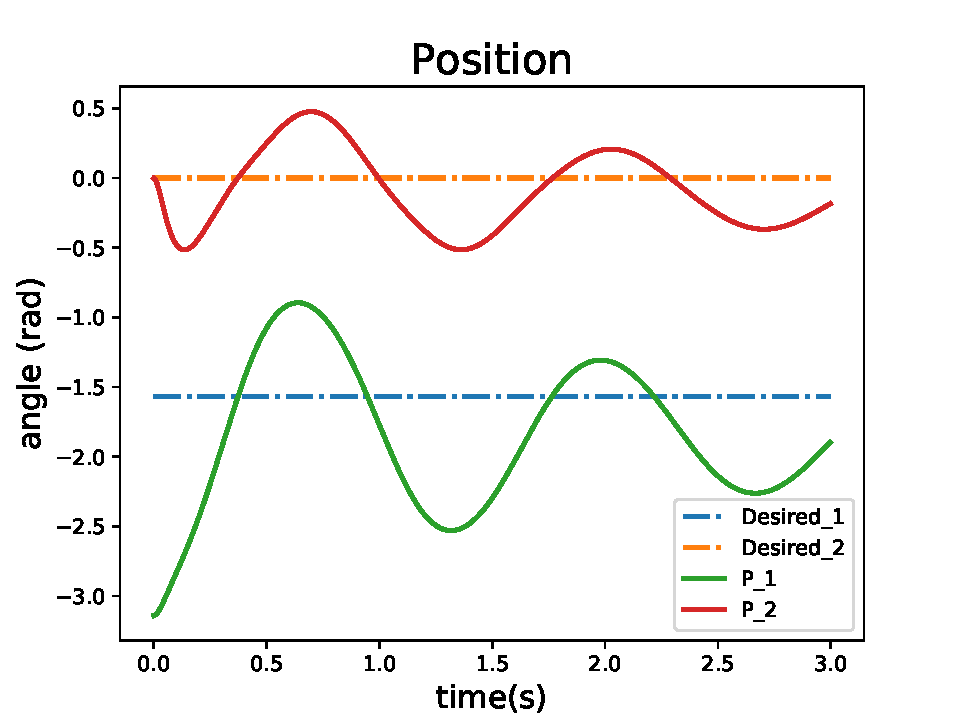
\includegraphics[width=.5\linewidth]{figures/P-Regler0.pdf}
%	\caption{Velocity Plot of a P-controller}
%	\label{P-Control}
%\end{subfigure}
%\begin{subfigure}%{width=.5\linewidth}
%	\centering
%	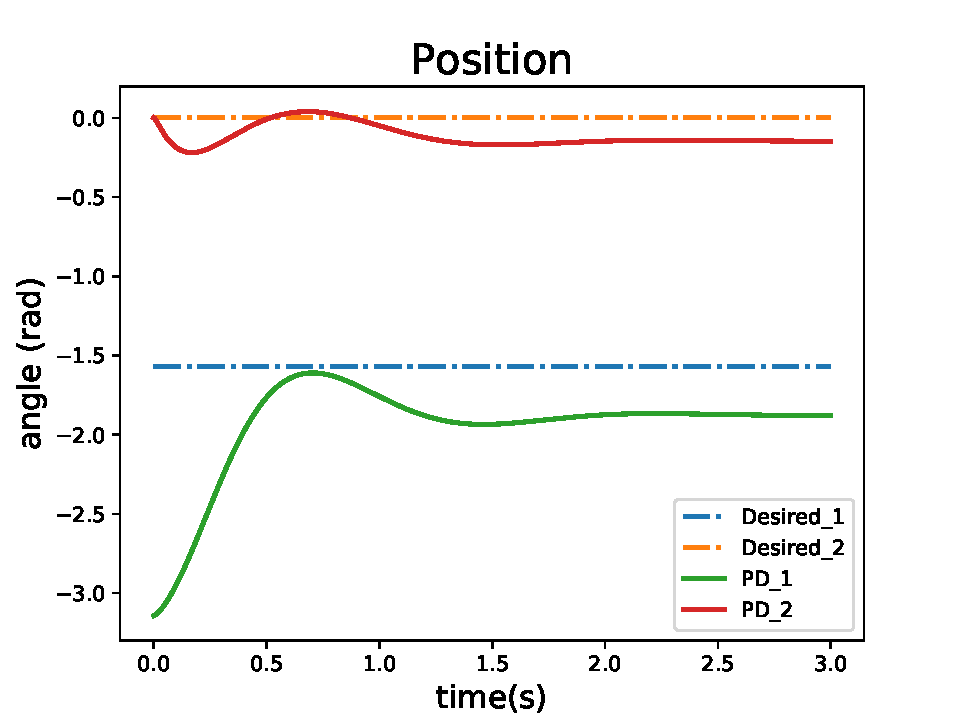
\includegraphics[width=.5\linewidth]{figures/PD-Regler0.pdf}
%	\caption{Velocity Plot of a PD-controller}
%	\label{PD-Control}
%\end{subfigure}
%	\caption{Velocitiy Plots of different controller}
%\end{figure}
\end{answer}
		
	\end{question}
	
	%----------------------------------------------
	
	\begin{question}{Tracking Trajectories}{4}
		Repeat the same experiment but this time use the provided time-varying target trajectory. Create (max 4) plots that compare the different control strategies and analyze the results. In your analysis discuss the overall performance and which controllers track the desired trajectory nicely. Additionally discuss which controller you would choose and why.
		
\begin{answer}
	\begin{center}
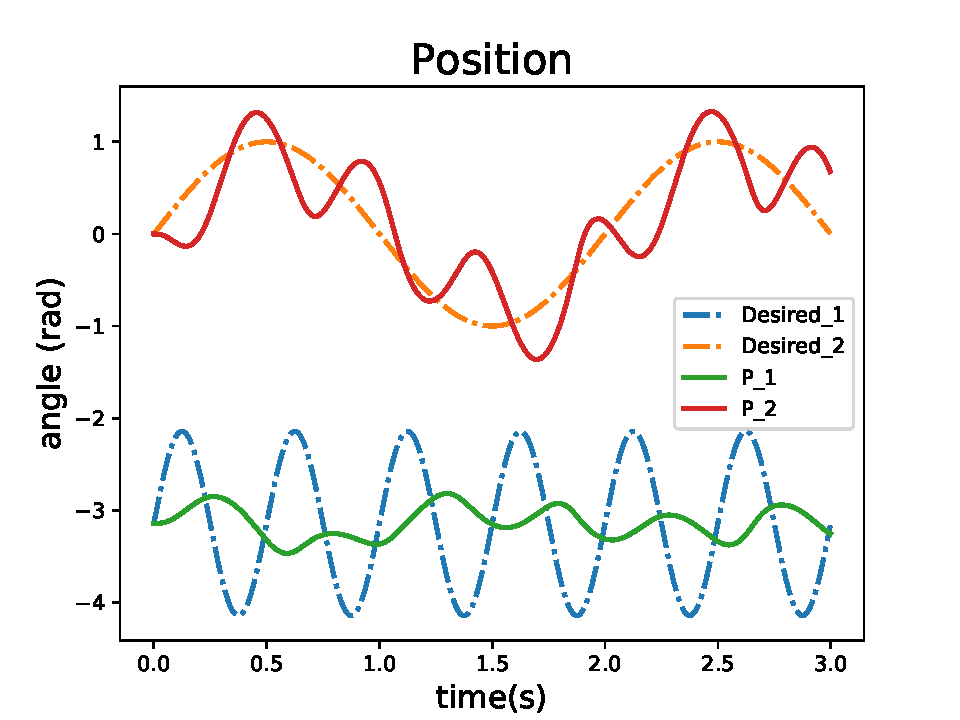
\includegraphics[width=.32\linewidth]{figures/P-traj0.pdf}
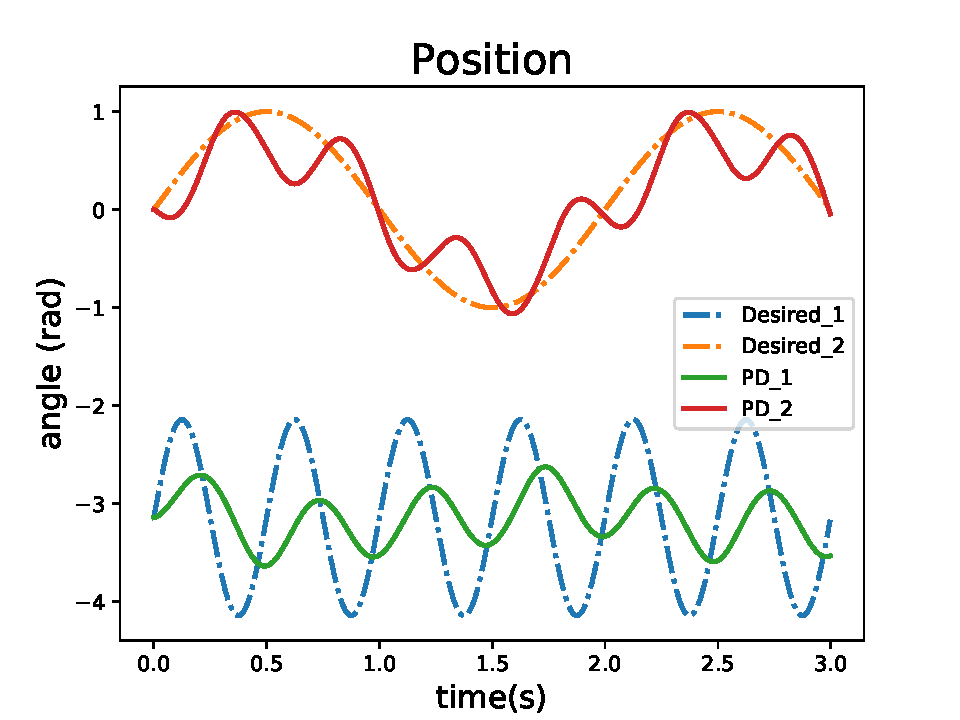
\includegraphics[width=.32\linewidth]{figures/PD-traj0.pdf}\\
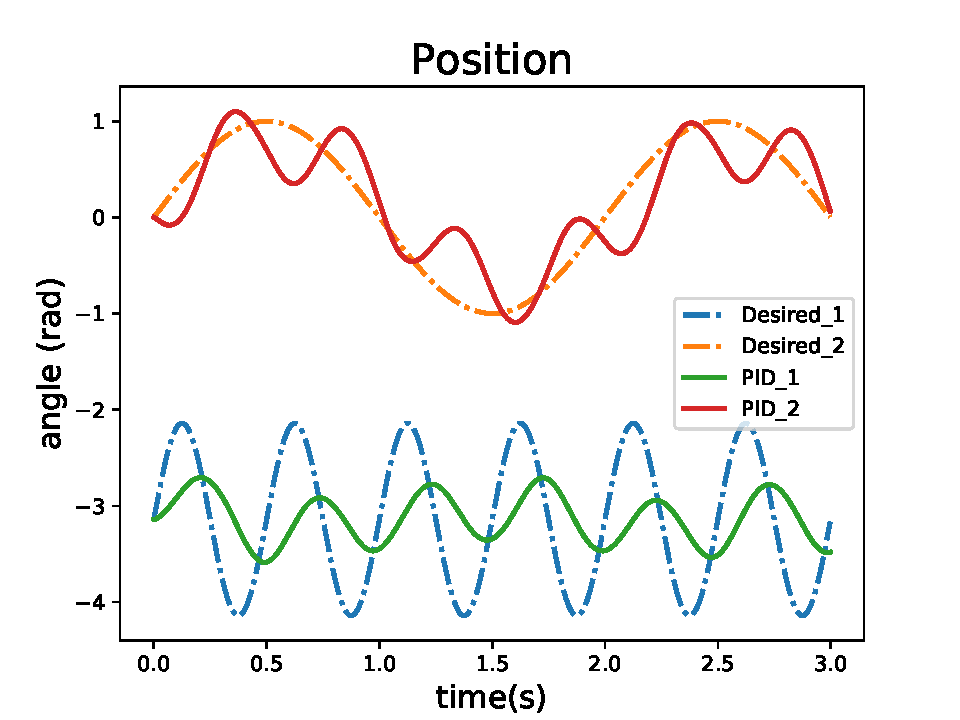
\includegraphics[width=.32\linewidth]{figures/PID-traj0.pdf}
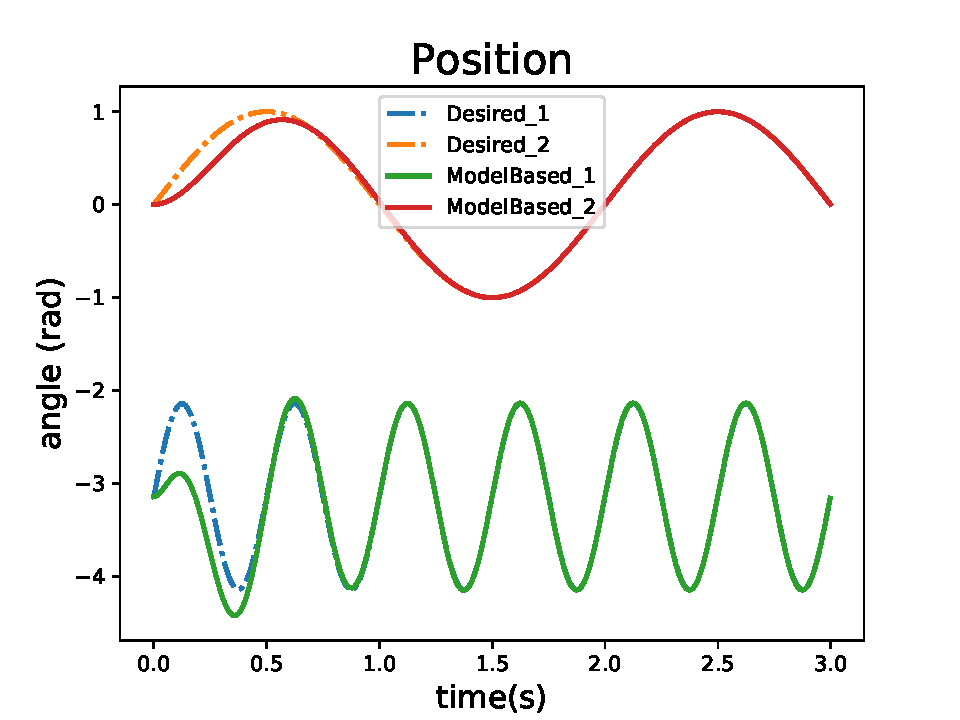
\includegraphics[width=.32\linewidth]{figures/Model-Based-traj0.pdf}
	\end{center}

While tracking the trajectory, all controllers behave in a similar way. the all oscilate around the wanted curve. The difference between them is very small, so even the PD controller which performed very well in the last task can't trace the trajectory very well. This behaviour is actually pretty bad compared to a model based controller, which fits the curve nearly perfect after just a little over half a second.
\end{answer}
		
	\end{question}
	
	%----------------------------------------------
	
	\begin{question}{Tracking Trajectories --- High Gains}{4}
		Repeat the same experiment (using the provided trajectory) but this time multiply the gains by ten. Create plots that compare the different control strategies and analyze the results. In your analysis discuss the overall performance and compare it to the previous case. Are there any drawbacks of using high gains?
		
\begin{answer}
%TODO
\end{answer}
		
	\end{question}
	
	%----------------------------------------------
	
	\begin{question}[bonus]{Task Space Control}{5}
		The robot must now reach a desired position in task space $\vec{x_\textrm{end}}={[-0.35,1.5]}$. In class we derived the Jacobian transpose, Jacobian pseudo-inverse, and Jacobian pseudo-inverse with damping methods. All of them are implemented in \texttt{my\_taskSpace\_ctl.py}. You are asked to implement also the null-space task prioritization method with a null-space resting posture $\vec q=[0,\pi]$. Run the simulation and plot the initial and final configuration of the robot. Then, change the resting posture to $\vec q=[0,-\pi]$ and redo the plots. Analyze in a couple of sentences your observation. Use the same damping coefficient $10^{-6}$ and include a code snippet to your solutions.
		
\begin{answer}
%TODO
\end{answer}
		
	\end{question}
	
\end{questions}


	
	\exercise{Machine Learning in a Nutshell}
For this exercise you will use a dataset, divided into training set and validation set (both attached). The first row is the vector $\vec x$ and the second row the vector $\vec y.$
\\
Based on these data, we want to learn a function mapping from $\vec x$ values to $\vec y$ values, of the form $\vec y=\vec{\theta}^{T}\vec{\phi}(\vec x)$.

For all questions requiring a plot, you also have to provide a snippet of your code!

You are allowed to use \texttt{scipy.spatial.distance.cdist} and \texttt{scipy.exp}.

\begin{questions}
	
	%----------------------------------------------
	
	\begin{question}{Supervised vs Unsupervised Learning}{2}
		Briefly explain the differences between supervised and unsupervised learning. 
		Is the above a supervised or unsupervised learning problem? Why?

\begin{answer}
%TODO :awful english 
supervised larning -> you get examples with solutions and learn based on these already completed examples.

unsupervised learning -> you learn via try and error. so you get a situaion or a training set without the soultion and have to learn yourself what works best. therefor you try out a lot of different hings and look what happens.

%TODO unsupervised?


\end{answer}
	\end{question}
	
	
	%----------------------------------------------
	
	\begin{question}{Regression vs Classification}{2}
		Supervised learning is typically divided into regression and classification tasks. 
		Briefly explain what are the differences between regression and classification.
		
\begin{answer}
	regression tasks: expected output, never mind how likely it is
	
	clasification tasks: most likely, never mind whats expected
	
	%TODO: On Slides_03 page 19
	
\end{answer}
\end{question}
	
	
	%----------------------------------------------
	
	\begin{question}{Linear Least Squares}{4}
		Consider the training set above to calculate features $\vec{\phi}(x)$ of the form $[\sin(2^{i}x)]_{i = 0 \ldots n-1}$. 
		Compute the feature values when $n$ is 2, 3 and 9 (i.e., when using 2, 3 and 9 features). 
		Use the linear least squares (LLS) method to predict output values $y$ for input values $x\in\{0, 0.01, 0.02, \ldots, 6\}$ using the different numbers of features. 
		Attach a single plot showing the three resulting predictions when using 2, 3 and 9 features (i.e., having $x$ and $y$ as axes).
		
\begin{answer}
%TODO
\end{answer}
		
	\end{question}
	
	
	%----------------------------------------------
	
	\begin{question}{Training a Model}{2}
		The root mean square error (RMSE) is defined as $\text{RMSE} = \sqrt{\frac{1}{N}\sum_{i=1}^{N}(y^{\text{true}}_i-y^{\text{predicted}}_i)^{2}}$, where $N$ is the number of data points. 
		Using the LLS algorithm implemented in the previous exercise, train a different model for each of the number of features between 1 and 9, i.e.,  [1,2,3...,9].
		For each of these models compute the corresponding RMSE for the training set. 
		Attach a plot where the x-axis represents the number of features and the y-axis represents the RMSE.
		
\begin{answer}
%TODO
\end{answer}
		
	\end{question}
	
	
	%----------------------------------------------
	
	\begin{question}{Model Selection}{4}
		Using the models trained in the previous exercise, compute the RMSE of each of these models for the validation set.\\
		Compare in one plot the RMSE on the training set and on the validation set. 
		How do they differ? 
		Can you explain what is the reason for these differences? (Hint: remember the plot from Exercise~c)~) 
		What is the number of features that you should use to achieve a proper modeling?
		
\begin{answer}
%TODO
\end{answer}
	\end{question}
	
	%----------------------------------------------
	
	\begin{question}{Cross Validation}{8}
		$K$-fold cross validation is a common approach to estimate the test error when the dataset is small.
		The idea is to randomly divide the training set into $K$ different datasets.
		Each of these datasets is then used as validation set for the model trained from the remaining $K-1$ datasets.
		The resulting vector of errors $\vec E = [ e_1... e_K ]$ can now be used to compute a distribution (typically by fitting a Gaussian distribution).
		When $K$ is equal to the number of data points, $K$-fold cross validation takes the name of leave-one-out cross validation (LOO).
		
		Apply LOO using only the training set and compute the mean/variance of the RMSE for the learned models. 
		Repeat for the models with the number of features between 1 and 9, i.e.,  [1,2,3...,9]
		
		Attach a plot showing the mean/variance (as a distribution) of the RMSE computed using LOO and having on the x-axis the number of features and on the y-axis the RMSE.
		Which is the optimal number of features now? 
		Discuss the results obtained and compare against model selection using train/validation set.
		
\begin{answer}
%TODO
\end{answer}
	\end{question}
	
	
	
	%----------------------------------------------
	
	
	\begin{question}{Kernel Functions}{2}
		A kernel function $k(\vec{\mbox{x}}_{i},\vec{\mbox{x}}_{j})$ is given by the inner product of two feature vectors. Write out the kernel function for the previous set of features where $n=3$.
		
\begin{answer}
%TODO
\end{answer}
	\end{question}
	
	
	%----------------------------------------------
	
	\begin{question}{Kernel Regression}{6}
		
		The kernel function in the previous question required explicit definition of the type and number of features, which is often difficult in practice. Instead, we can use a kernel that defines an inner product in a (possibly infinite dimensional) feature space. \\
		Using the training set and an exponential squared kernel 		$k( \vec{x}_{i} , \vec{x}_{j} )= \exp ( -\frac{1}{\sigma^{2}} \Vert \vec{x}_{i}-\vec{x}_{j}\Vert ^{2} )$ with $\sigma=0.15$, predict output values $y$ for input values $x\in\{0,0.01,\ldots,6\}$. Attach a plot of your results.
		\\
		(Hint: use standard kernel regression: $f(\mbox{\ensuremath{\vec{x}}})=\vec{k}\T\vec{K}^{-1}\vec{y}$ with $\vec{K}_{ij}=k(\vec{x}_{i},\vec{x}_{j})$ and $\vec{k}_{i}=k(\vec{x},\vec{x}_{i})$).
		
		Compute the RMSE on the validation set for the kernel regression model. Compare it with the RMSE of the best LLS model you found.
		
\begin{answer}
%TODO
\end{answer}
	\end{question}
	
	
	%----------------------------------------------
	
	\begin{question}[bonus]{Derivation}{5}
		Explain the concept of ridge regression and why/when it is used.
		Derive its final equations presented during the lecture.\\
		(Hint: remind that for normal linear regression the cost function is $J = \frac{1}{2}\sum_{i=1}^N ( f(\vec x_i) - y_i ) ^2 \,$ )\\
		(Hint 2: use matrix notation)
		
\begin{answer}
%TODO
\end{answer}
	\end{question}	
	
\end{questions}


	
\end{document}

